% !TEX root = ../main.tex

\section{Experimental Results}
\label{sec:orgc23a664}

We present classification results on four different datasets, movie\-Posters, cancerHallmarks, chemicalExposure and arXiv2020 in Table~\ref{table:overallresults}. 

\subsection{Overall classification results}

In general, we observe that the sigmoidF1 loss performs better on most metrics and across different datasets. In particular, sigmoidF1 always outperforms other losses on the metric on which focus (weightedF1 @ 0.5) and its non-weighted counterpart (microF1 @ 0.5). 
On the moviePosters dataset (Table~\ref{tab:moviePosters}) and the arXiv2020 dataset (Table~\ref{tab:arxiv2020}), we observe higher scores for the sigmoidF1 loss on all but Precision @ 0.5. 
On the smaller chemicalExposure and cancerHallmarks datasets, the unboundedF1 loss delivers good results for macroF1 @ 0.5 and Precision @ 0.5 and the sigmoidF1 loss leads to higher scores on the remainder of the metrics.

% \todo{Note that contrary to sigmoidF1, unboundedF1 can be particularly performant without requiring hyperparameter tuning.}\daan{Not a very strong point for sigmoidF1. Also not sure if I agree. We focus on weightedF1, that we hopefully succesfully defended in 4. We see substantial improvements for sigmoidF1 over softF1 across the board on that metric. So we should explain that we see that it optimized for a macro metric instead and clearly has success that. Can be a strong metric to consider for such a setting. That should be its on paragraph.}

% \gab{comment on 0.0 CE for cancer}

FocalLoss, which is specifically tailored for sparse data, does not perform well in our experiments, except for the Precision @ 0.5 metric on the moviePosters dataset. This can be explained by the fact that FocalLoss is designed for multi-class uni-label problems. 
% We have already said the following:
%Across Tables~\ref{tab:moviePosters}, \ref{tab:arxiv2020}, \ref{tab:cancerHallmarks} and \ref{tab:chemicalExposure} we see that the smooth sigmoidF1 loss outperforms other existing losses.

\begin{table*}
\caption{Multi-label classification performance@0.5.}
\label{table:overallresults}
\vspace{2mm}
\begin{subtable}[t]{.95\columnwidth}
  \caption{MobileNetV2 (CNN) + classification head on the moviePosters dataset.}
  \label{tab:moviePosters}
\centering
\begin{tabular}{l ccccc}
\toprule 
Loss  & \rotatebox{45}{weightedF1} & \rotatebox{45}{microF1} & \rotatebox{45}{macroF1} & \rotatebox{45}{Precision}\\% & \rotatebox{90}{Recall}\\ 
\midrule
$\mathcal{L}_{\text {CE}}$ & 0.149 & 0.186 & 0.051 & 0.090\\% & 0.042 \\
$\mathcal{L}_{\text {FL}}$ & 0.154 & 0.192 & 0.055 & 0.115\\% & – \\
% $\mathcal{L}_{\text {CE+N}}$ & 0 & 0 & 0 & 0 & 0 \\
$\mathcal{L}_{\text {unboundedF1}}$ & 0.243 & 0.207 & 0.136 & \textbf{0.105}\\% & 0.190 \\
$\mathcal{L}_{\text {sigmoidF1}}$ & \textbf{0.300} & \textbf{0.224} & \textbf{0.158} & 0.104\\% & \textbf{0.557} \\ % run aa424792a57e4208ad1805cd6e63f8e6
\bottomrule
\end{tabular}
\end{subtable}
\quad
\begin{subtable}[t]{.95\columnwidth}
  \caption{DistilBert (NLP) + classification head on  the arXiv2020 dataset.}
  \label{tab:arxiv2020}  
\centering
\begin{tabular}{l ccccc}
\toprule
Loss  & \rotatebox{45}{weightedF1} & \rotatebox{45}{microF1} & \rotatebox{45}{macroF1} & \rotatebox{45}{Precision}\\% & \rotatebox{90}{Recall}\\ 
\midrule
$\mathcal{L}_{\text {CE}}$ & 0.106 & 0.106 & 0.093 & 0.096\\% & – \\ % Run 71ef078f975649d5b3d897e504bc638b
$\mathcal{L}_{\text {FL}}$ & 0.009 & 0.011 & 0.008 & 0.054\\% & 0.954 \\
% $\mathcal{L}_{\text {CE+N}}$ & 0 & 0 & 0 & 0 & 0 \\
$\mathcal{L}_{\text {unboundedF1}}$ & 0.087 & 0.088 & 0.077 & \textbf{0.100}\\% & – \\ % run 405a6e6851e84a89a82313251a7a36e8 (18-19 jan)
$\mathcal{L}_{\text {sigmoidF1}}$ & \textbf{0.106} & \textbf{0.106} & \textbf{0.093} & 0.096\\% & \textbf{–} \\ % run bd478ca55eb64cc78d9ad0f25accce35 (18-19 jan)
\bottomrule
\end{tabular}
\end{subtable}

\vspace{2mm}
\begin{subtable}[t]{.95\columnwidth}
  \caption{DistilBert (NLP) + classification head on the cancerHallmarks dataset.}
  \label{tab:cancerHallmarks}
\centering
\begin{tabular}{l ccccc}
\toprule 
Loss  & \rotatebox{45}{weightedF1} & \rotatebox{45}{microF1} & \rotatebox{45}{macroF1} & \rotatebox{45}{Precision}\\% & \rotatebox{90}{Recall}\\ 
\midrule
$\mathcal{L}_{\text {CE}}$ & 0.0 & 0.0 & 0.0 & 0.0 &\\% 0.0 \\ 
$\mathcal{L}_{\text {FL}}$ & 0.108 & 0.190 & 0.044 & 0.071 &\\% 0.055 \\
% $\mathcal{L}_{\text {CE+N}}$ & 0 & 0 & 0 & 0 & 0 \\
$\mathcal{L}_{\text {unboundedF1}}$ & 0.170 & 0.176 & \textbf{0.098} & \textbf{0.089}\\% & 0.131 \\
$\mathcal{L}_{\text {sigmoidF1}}$ & \textbf{0.202} & \textbf{0.313} & 0.095 & 0.059\\% & \textbf{0.264} \\ % run e145056949424b02bfc83cc57af38374
\bottomrule
\end{tabular}
\end{subtable}
\quad
\begin{subtable}[t]{.95\columnwidth}
  \caption{DistilBert (NLP) + classification head on the chemicalExposure dataset.}
  \label{tab:chemicalExposure}
\centering
\begin{tabular}{l ccccc}
\toprule
Loss  & \rotatebox{45}{weightedF1} & \rotatebox{45}{microF1} & \rotatebox{45}{macroF1} & \rotatebox{45}{Precision}\\% & \rotatebox{90}{Recall}\\ 
\midrule
$\mathcal{L}_{\text {CE}}$ & 0.051 & 0.058 & 0.012 & 0.047\\% & 0.007 \\ % Run 71ef078f975649d5b3d897e504bc638b
$\mathcal{L}_{\text {FL}}$ & 0.268 & 0.348 & 0.0934 & 0.130\\% & 0.091 \\
$\mathcal{L}_{\text {unboundedF1}}$ & 0.218 & 0.194 & \textbf{0.133} & \textbf{0.155}\\% & 0.138 \\ % run 405a6e6851e84a89a82313251a7a36e8 (18-19 jan)
$\mathcal{L}_{\text {sigmoidF1}}$ & \textbf{0.319} & \textbf{0.432} & 0.113 & 0.091\\% & \textbf{0.188} \\ % run a30825efe9c94a24bc46a9c71a5f8646 E: 0.5 S: 0.6
\bottomrule
\end{tabular}
\end{subtable}
\end{table*}


\subsection{Sensitivity analysis}

In Figure \ref{fig:betaEta} we show the sensitivity of sigmoidF1 to different parametrizations of $\eta$ and $\beta$. It is clear from Figure \ref{fig:betaEta} that results on the test set are quite sensitive to the choice of $\eta$ and $\beta$. Within the sampled values (see Section~\ref{subsec:hypers}), we chose to display a parameter space similar to the one illustrated in Figure~\ref{fig:sigmoid}. Moving the sigmoid to the left allows the learning algorithm to tend to a (local) optimum.

In general and across datasets, when sampling for $\eta$, we noticed how the optimum tended towards positive values. Offsetting the sigmoid curve to the left has the effect of pushing more candidate predictions to the rank of positive instance (or at least close to 1). We also note how $\beta$ (which cannot be negative or otherwise the sigmoid function would flip around the horizontal axis) is at best close to a value close to 0 on this dataset (we show discrete values here for display purposes). The sigmoid is thus relatively flat, which involves dynamic gradients over different batches. The idea is similar to a high learning rate. In our experiments, this rarely lead to divergent behavior in the loss function (learning curve).

% \subsection{\mdr{What's here?}}

% We perform an analysis of sensitivity to different amounts of labels. For this, the irrelevance threshold (see definition in Section \ref{sec:orgb44ba25}) $t$ was set to the values 0, 10, 100 and 1000. This time, results are shown with dichotomization thresholds of 0.1 to 0.9. \todo{see if keep it}

% \begin{figure}[htbp]
% \centering
% 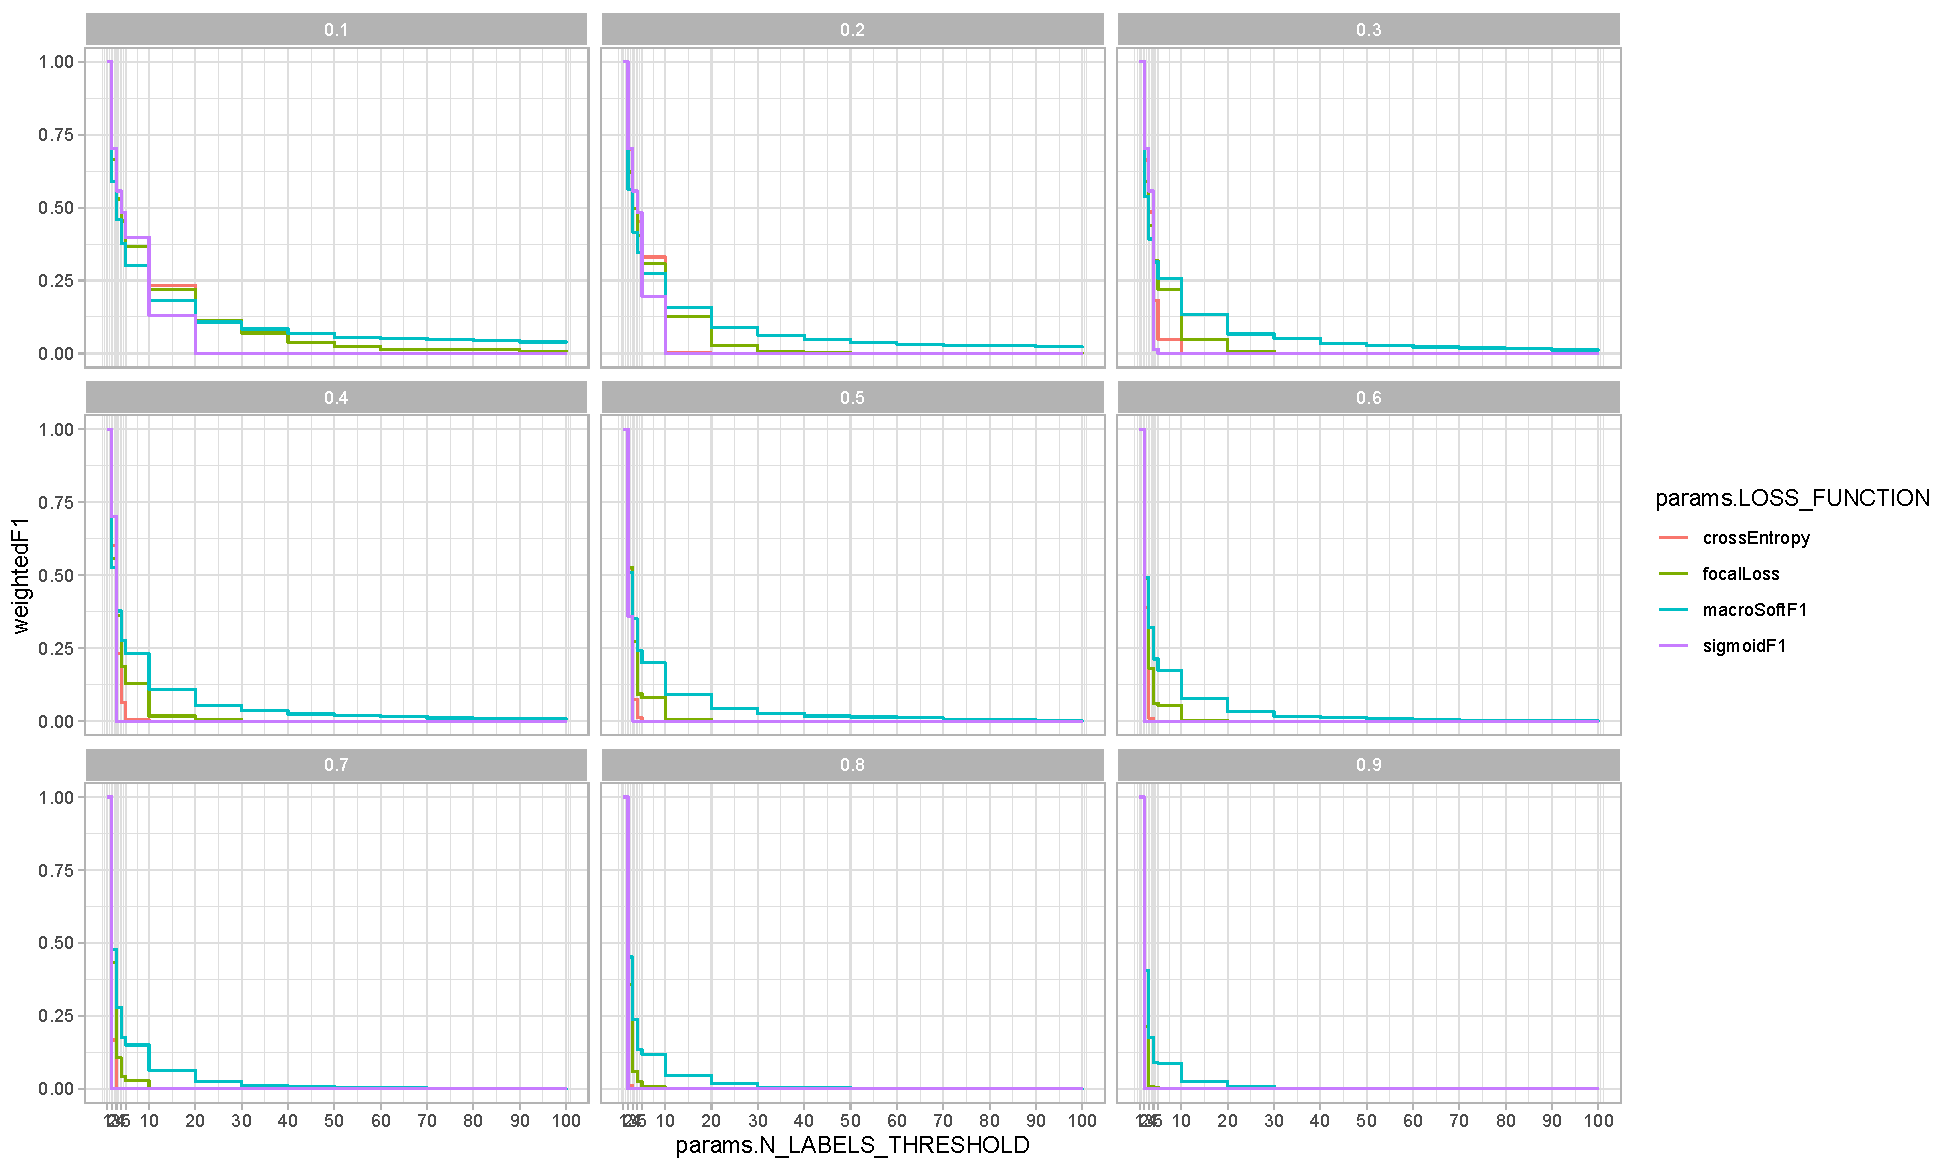
\includegraphics[width=.9\linewidth]{./images/ablation.pdf}
% \caption{\label{fig:ablation}
% Sigmoid function with different values for $\beta$ (steepness) \& $\eta$ (offset)}
% \end{figure}




%%% Local Variables:
%%% mode: latex
%%% TeX-master: "../main"
%%% End:
